\documentclass[11pt]{article}

\usepackage[T1]{fontenc}		% use this if European fonts (ec) package is installed
\usepackage{textcomp}			% adds some additional symbols
\usepackage[scaled=0.92]{helvet}	% set Helvetica as the sans-serif font
\renewcommand{\rmdefault}{ptm}		% set Times as the default text font

\usepackage{amsmath}
\usepackage{mathtools} % fix bugs in amsmath, provide \mathrlap etc.
\usepackage{hyperref} 
\usepackage{graphicx}
\usepackage[bf,small]{caption}
\usepackage{cite} % Compress consecutive citations
% The following loads mtpro and defines some common MTPro options [2, 4]
%\usepackage[subscriptcorrection,slantedGreek,nofontinfo,mtpccal,amssymbols]{mtpro2}
\usepackage[slantedGreek,nofontinfo,mtpccal,amssymbols]{mtpro2}

%\usepackage{units}
\usepackage{tikz}
\usetikzlibrary{patterns}


\newcommand{\fref}[1]{Fig.~\ref{#1}}

\newcommand{\x}{\boldsymbol{\hat{x}}}
\newcommand{\y}{\boldsymbol{\hat{y}}}
\newcommand{\z}{\boldsymbol{\hat{z}}}
\newcommand{\cross}{\boldsymbol{\times}}
\newcommand{\mat}[1]{\boldsymbol{\cal{#1}}}

\newcommand{\E}{\boldsymbol{E}}
\newcommand{\EI}{\E^{\text{I}}}
\newcommand{\EII}{\E^{\text{II}}}
\renewcommand{\H}{\boldsymbol{H}}
\newcommand{\HI}{\H^{\text{I}}}
\newcommand{\HII}{\H^{\text{II}}}
\newcommand{\e}{\boldsymbol{e}}
\newcommand{\enorm}{\boldsymbol{\varepsilon}}
\newcommand{\h}{\boldsymbol{h}}
\newcommand{\f}{\boldsymbol{f}\mkern-4mu}
\newcommand{\I}{\ensuremath{\text{I}}}
\newcommand{\II}{\ensuremath{\text{II}}}
\newcommand{\eI}{\e^{\text{I}}}
\newcommand{\eII}{\e^{\text{II}}}
\newcommand{\hI}{\h^{\text{I}}}
\newcommand{\hII}{\h^{\text{II}}}
\newcommand{\MI}{M_{\text{I}}}
\newcommand{\MII}{M_{\text{II}}}
\newcommand{\aI}{a^{\text{I}}}
\newcommand{\avecI}{\mat{a}^{\text{I}}}
\newcommand{\avecII}{\mat{a}^{\text{II}}}
\newcommand{\bvecI}{\boldsymbol{b}^{\text{I}}}
\newcommand{\bvecII}{\boldsymbol{b}^{\text{II}}}
\newcommand{\aII}{a^{\text{II}}}
\newcommand{\bI}{b^{\text{I}}}
\newcommand{\bII}{b^{\text{II}}}
\newcommand{\gammaI}{\gamma^{\text{I}}}
\newcommand{\gammaII}{\gamma^{\text{II}}}
\newcommand{\transpose}{^\text{\sf T}}
\newcommand{\diag}{\operatorname{diag}}
\newcommand{\colvec}[1]{\begin{bmatrix} #1 \end{bmatrix}}
\newcommand{\phihat}{\boldsymbol{\hat{\phi}}}
\newcommand{\thetahat}{\boldsymbol{\hat{\theta}}}
\newcommand{\rhohat}{\boldsymbol{\hat{\rho}}}
\renewcommand{\r}{\boldsymbol{r}}
\newcommand{\rhat}{\boldsymbol{\hat{r}}}
\newcommand{\Rin}{R_{\text{in}}}
\newcommand{\Rout}{R_{\text{out}}}
\newcommand{\wlmin}{\lambda_{\text{min}}}
\newcommand{\TE}{\text{TE}}
\newcommand{\TM}{\text{TM}}
\newcommand{\psq}{^{\prime \,\raisebox{0.2ex}{$\scriptstyle2$}}}
\newcommand{\Nmode}{{N_{\text{m}}}}
\newcommand{\J}{\boldsymbol{J}}
\newcommand{\Jtilde}{\tilde{\mkern -2mu\J\mkern 2mu}}
\newcommand{\M}{\boldsymbol{M}}
\newcommand{\Mtilde}{\tilde{\mkern -2mu\M\mkern 2mu}}
\newcommand{\A}{\boldsymbol{A}}
\newcommand{\F}{\boldsymbol{F}}
\newcommand{\hermitian}{^{\text{\sffamily H}}}
\newcommand{\hhat}{\boldsymbol{\hat{h}}}
\newcommand{\vhat}{\boldsymbol{\hat{v}}}
\newcommand{\Rx}{R_{x}} \newcommand{\phix}{\gamma_{x}}
\newcommand{\Rz}{R_{z}} \newcommand{\phiz}{\gamma_{z}}
\newcommand{\Rhat}{\boldsymbol{\hat{R}}}
\newcommand{\Lhat}{\boldsymbol{\hat{L}}}
\newcommand{\norm}[1]{\lVert #1 \rVert} % Norm operator
\newcommand{\abs}[1]{\lvert #1 \rvert} % absolute value operator


\allowdisplaybreaks[1]





\begin{document}

\title{\bfseries GSM Analysis of TE$_{\boldsymbol{1}\boldsymbol{1}\boldsymbol{p}}$ Mode Cylindrical Cavity}
\author{Peter S.\ Simon}        
\date{4 June 2025}
\maketitle
This document is licensed under the Creative Commons Attribution 4.0 International License.
To view a copy of this license, visit \url{http://creativecommons.org/licenses/by/4.0/}
or send a letter to Creative Commons, PO Box 1866, Mountain View, CA 94042, USA. 


\hyphenation{wave-guide}
\hyphenation{wave-guides}


\section{Introduction}
\label{sec:intro}
The purpose of these notes is to document a method to rapidly and accurately compute transmission amplitude for
a resonant cavity like that shown in \fref{fig:structure}.  At one end of the cavity, following
a transition from rectangular to circular guide, is a thin annular, metal
spacer (shown in gray in the figure). It has the effect of slightly reducing the inner radius of the circular
waveguide comprising the body of the cavity. This region of reduced radius is labeled ``CWG I'' in part (b)
of the figure. Following the spacer, in the slightly larger radius guide,
is a thin disk of dielectric material (shown in yellow in part (a) of the figure),
followed by a region of empty guide (``CWG II'') terminated with a final transition to rectangular guide.
%
\begin{figure}
  \centering
  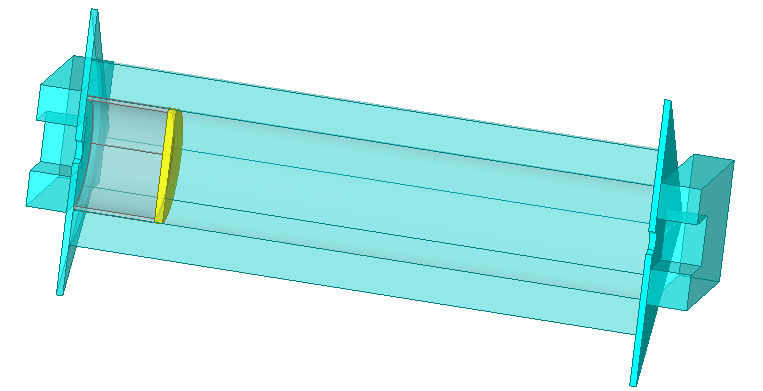
\includegraphics[scale=0.4]{CAD_image.png} \\ (a)
  \\[\baselineskip]
  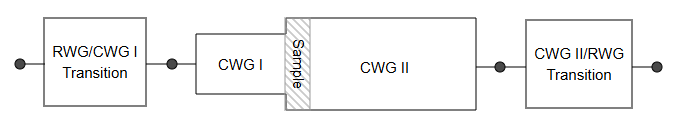
\includegraphics[scale=0.6]{schematic_diagram.png} \\ (b)
  \caption{The structure to be analyzed: (a) Cutaway view of 3D model. (b) Schematic.}
    \label{fig:structure}
\end{figure}

The structure will be analyzed by cascading the generalized scattering matrices (GSMs) that characterize
each discontinuity and each region of uniform waveguide. For most of the structure, it will be sufficient
to track only a single waveguide mode, the TE$_{11}$ mode.  But for the radius step followed by the thin
dielectric disk, a full multi-modal GSM analysis will be used. This is illustrated in \fref{fig:fullschematic}.
%
\begin{figure}
  \centering
  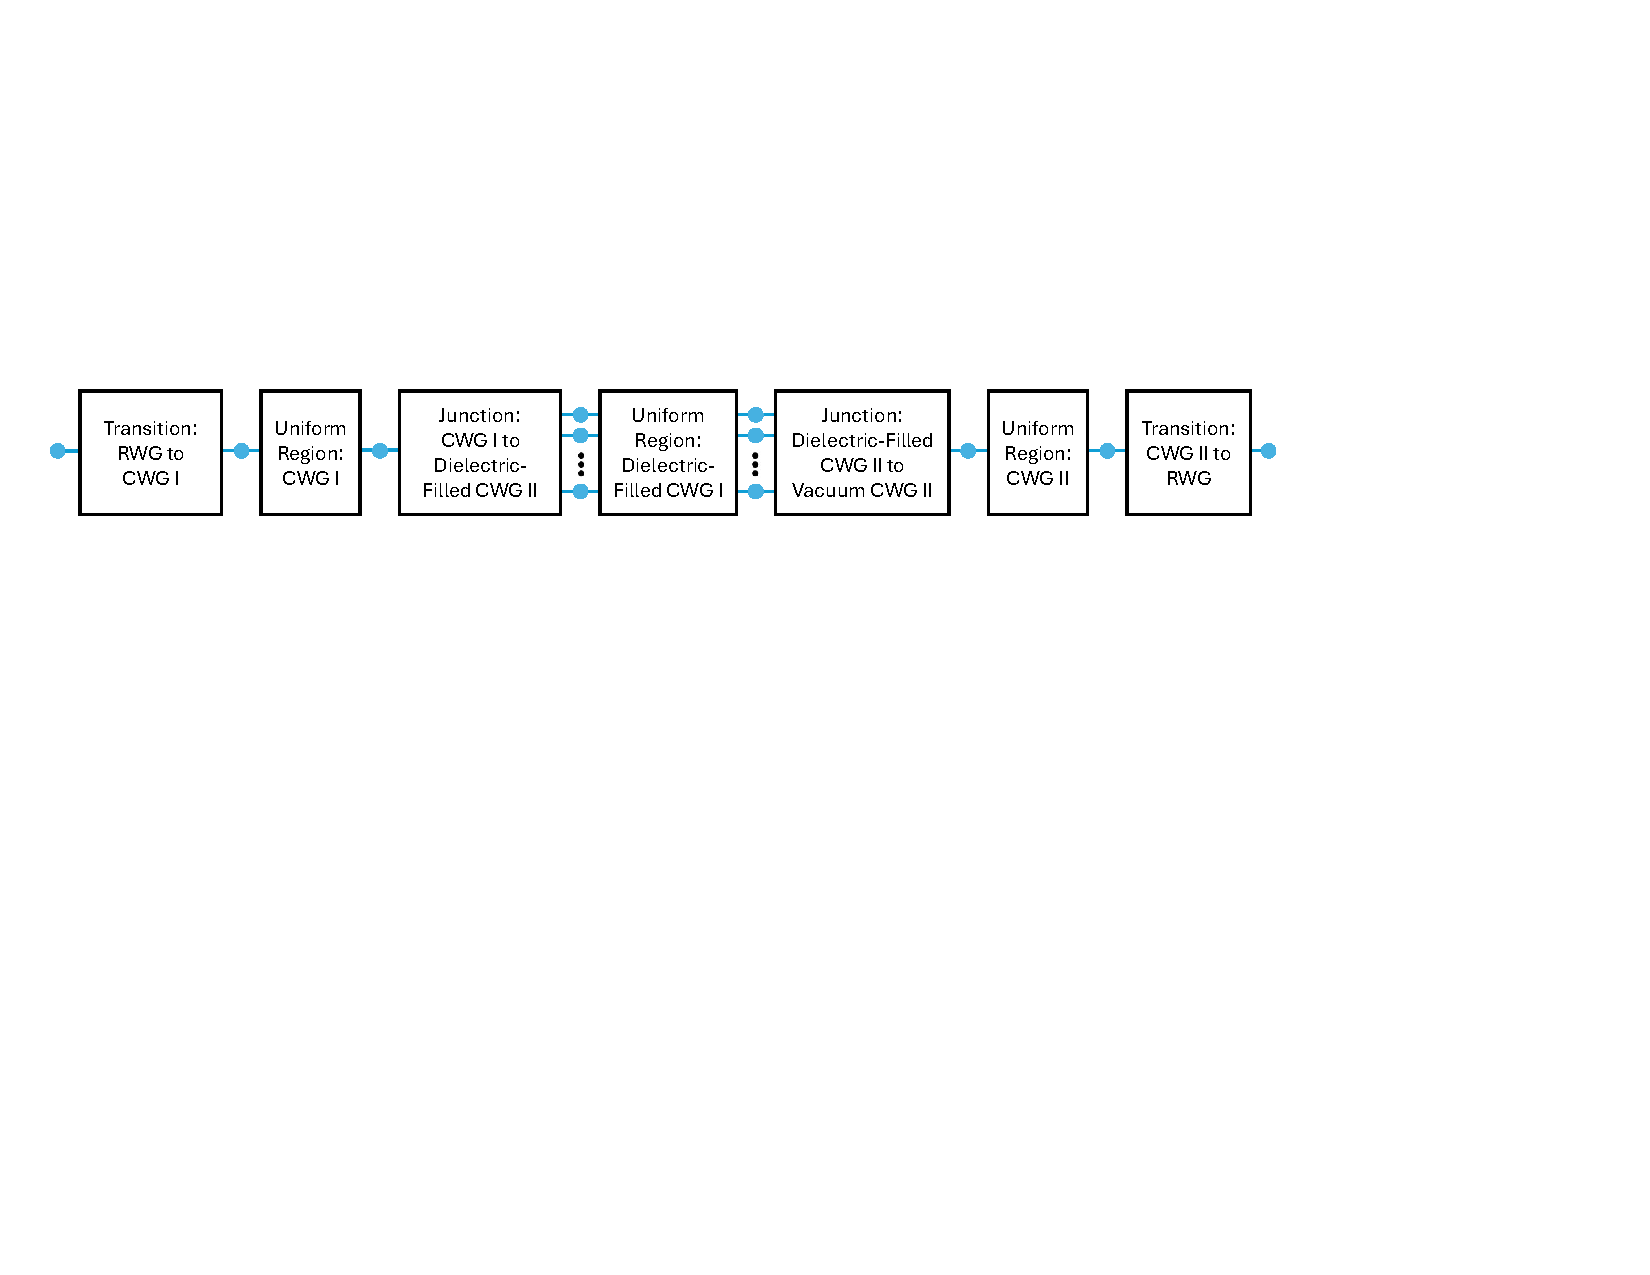
\includegraphics[angle=90,origin=c,scale=0.8]{full_schematic.pdf}
  \caption{Diagram illustrating each GSM network to be cascaded.  Single-mode $2\times2$ scattering matrices are
  shown as 2-port networks.}
    \label{fig:fullschematic}
\end{figure}


\section{Theory}
\label{sec:theory}


\subsection{Mode Matching at a Junction of Two Circular Waveguides}
\label{sec:modematch}
In this section we restrict consideration to the junction of a pair of semi-infinite circular waveguides,
which may be filled with different materials.
The mode matching formulation developed here most closely
follows the notation of James \cite{jame:81}.
We assume that the structure is excited at either end by an incident field
consisting of a single $\TE_{11}$ mode, so that only $m=1$ modes as
defined in Appendix~\ref{app:modes} can exist at any location in the
structure. For these modes, the azimuthal variation is limited to be
proportional to either $\cos\phi$ or $\sin\phi$.

In the interior of either uniform CWG segment, the entire (finite) set of
TE and TM $m=1$ modes under consideration is sorted into order of
increasing cutoff frequency and the modes in this set are indexed using
a single natural number, say, $m$.
The modes are orthogonal and normalized in accordance with
\eqref{eq:normalization}. 


The two uniform CWGs are concentric
with the $z$-axis, of radii $R_{\I}$ and $R_{\II} \ge R_{\I}$.  The
junction occurs at the $z=0$ plane and the waveguide with smaller
(larger) radius occupies the half-space $z<0$ ($z>0$). 

Near the junction the transverse fields in Region~I ($z<0$) are
written as a sum of the modes of waveguide~I:
\begin{subequations}
\label{eq:13}
  \begin{align}
    \EI(\rho,\phi,z) &= \sum_{m=1}^{\MI} (\aI_m e^{-\gammaI_m z} + \bI_m
    e^{\gammaI_m z})  \eI_m(\rho,\phi) \\
    \HI(\rho,\phi,z) &= \sum_{m=1}^{\MI} (\aI_m e^{-\gammaI_m z} - \bI_m
    e^{\gammaI_m z})  \hI_m(\rho,\phi).
  \end{align}
\end{subequations}
For Region~II ($z>0$), we again write the fields in terms of incident and
reflected traveling waves:
\begin{subequations}
\label{eq:14}
\begin{align}
    \EII(\rho,\phi,z) &= \sum_{m=1}^{\MII} (\aII_m e^{\gammaII_m z} + \bII_m
    e^{-\gammaII_m z})  \eII_m(\rho,\phi), \\
    \HII(\rho,\phi,z) &= \sum_{m=1}^{\MII} (-\aII_m e^{\gammaII_m z} + \bII_m
    e^{\gammaII_m z})  \hII_m(\rho,\phi).
  \end{align}
\end{subequations}

To find the scattering matrix of the junction, we enforce the equality
of the tangential electric and magnetic fields in a weighted average sense,
using the modes of the larger guide as testing or weighting functions.  First the
continuity of tangential electric field is tested. In the
following, the disk of radius $R$ is denoted as $C_{R}$.
\begin{multline}
  \label{eq:12}
  \iint_{C_{R_\I}}\mkern-12mu \EI(x,y,0) \cross   \hII_m(\rho,\phi) \cdot \z \, dS
  = 
  \iint_{C_{R_\I}}\mkern-12mu \EII(x,y,0) \cross  \hII_m(\rho,\phi) \cdot \z \, dS
  \\ = 
  \iint_{C_{R_\II}}\mkern-12mu \EII(x,y,0) \cross \hII_m(\rho,\phi) \cdot \z \, dS.
\end{multline}
The final equality in \eqref{eq:12} above follows from the fact that
the tangential electric field $\EII(x,y,0)$ is zero over the region
$C_{R_\II} - C_{R_\I}$ so that the integral can be extended over the larger
disk. Inserting \eqref{eq:13} and \eqref{eq:14} into \eqref{eq:12}
and using the orthogonality of the modes yields
\begin{equation}
  \label{eq:15}
  \sum_{n=1}^{\MI} \bigl(\aI_n + \bI_n\bigr) P_{mn} = \aII_m + \bII_m,
  \quad m = 1, 2, \ldots, \MII,
\end{equation}
where
\begin{equation}
  \label{eq:16}
  P_{mn} =    
  \iint_{C_{R_{\I}}} \mkern-12mu \eI_n \cross \hII_m \cdot \z \, dS.
\end{equation}


Next, we enforce continuity of tangential magnetic field over the
common aperture:
\begin{equation}
  \iint_{C_{R_\I}} \mkern-12mu \eI_m \cross \HI(x,y,0) \cdot \z \, dS
  =
  \iint_{C_{R_\I}} \mkern-12mu \eI_m \cross \HII(x,y,0) \cdot \z \, dS
\end{equation}
which, upon expanding the fields into modal series and invoking
orthogonality, yields
\begin{equation}
  \label{eq:17}
  \aI_m - \bI_m = 
  \sum_{n=1}^{\MII} \bigl(\bII_n - \aII_n\bigr) P_{nm}, \quad m = 1,
  2, \ldots, \MI.
\end{equation}
Equations~\eqref{eq:15} and \eqref{eq:17} can be written in matrix
form as follows:
\begin{gather}
  \label{eq:18}
  \mat{P} (\avecI + \bvecI) = \avecII + \bvecII \\
  \label{eq:19}
  \avecI - \bvecI = \mat{P}\transpose (\bvecII - \avecII),
\end{gather}
where $\mat{P}\transpose$ is the transpose of $\mat{P}$.  Multiplying
\eqref{eq:19} by $\mat{P}$ and adding the result to \eqref{eq:18}
eliminates $\bvecI$ and allows one to solve for $\bvecII$ in terms of
$\avecI$ and $\avecII$.  Similarly, multiplying \eqref{eq:18} by
$\mat{P}\transpose$ and subtracting the result from \eqref{eq:19}
eliminates $\bvecII$ and allows one to solve for $\bvecI$ in terms of
$\avecI$ and $\avecII$.  After performing these operations, one can
write the generalized\footnote{``Generalized'' because it also
  includes scattering coefficients for cut-off modes.}
 scattering relation of the junction as 
\begin{equation}
  \label{eq:20}
  \colvec{\bvecI \\ \bvecII} = 
  \begin{bmatrix}
    \mat{S}^{\I,\I} & \mat{S}^{\I,\II} \\
    \mat{S}^{\II,\I} & \mat{S}^{\II,\II} 
  \end{bmatrix}
  \colvec{\avecI \\ \avecII} 
\end{equation}
where
\begin{subequations}
  \label{eq:21all}
\begin{align}
  \label{eq:21}
  \mat{S}^{\I,\I} &= (\mat{I} + \mat{P}\transpose\mat{P})^{-1}
  (\mat{I} - \mat{P}\transpose\mat{P}),
  \\
  \mat{S}^{\I,\II} &= 2(\mat{I} + \mat{P}\transpose\mat{P})^{-1}
  \mat{P}\transpose,
  \\
  \mat{S}^{\II,\I} &= 2(\mat{I} + \mat{P}\mat{P}\transpose)^{-1}
  \mat{P},
  \\
  \mat{S}^{\II,\II} &= -(\mat{I} + \mat{P}\mat{P}\transpose)^{-1}
  (\mat{I} - \mat{P}\mat{P}\transpose),
\end{align}
\end{subequations}
and $\mat{I}$ is the identity matrix.  Since the scattering matrix of
a waveguide junction is symmetric, we must have that $\mat{S}^{\I,\I}$
and $\mat{S}^{\II,\II}$ are symmetric matrices, and that
$\mat{S}^{\II,\I}$ is the transpose of ${\mat{S}^{\I,\II}}$.


\subsubsection{Efficient Evaluation of the Mode Coupling Coefficients}
The scattering matrices in \eqref{eq:21all} will be required at many
different frequencies. It is possible to compute a universal set of 
coupling coefficients that can be used for any frequency. The procedure for doing so is
outlined in this section.

We begin with \eqref{eq:16}, writing the integrand in terms of the
modal electric fields:
\begin{align}
  \label{eq:22}
  P_{mn} &=  
  \iint_{C_{R_{\I}}} \mkern-12mu \eI_n \cross \hII_m \cdot \z \, dS 
  = Y^\II_m
  \iint_{C_{R_{\I}}} \mkern-12mu \eI_n(\rho,\phi) \cdot \eII_m(\rho,\phi) \, dS. 
\end{align}
We now define the unit radius, frequency-independent modal fields
$\enorm^{\TE}_{mn}$ and $\enorm^{\TM}_{mn}$ to be the
$mn$th TE or TM modal electric field that would exist in a unit radius
waveguide, divided by the square root of the modal impedance.
From the formulas of Appendix~\ref{app:modes} we see that the explicit
forms of the frequency-independent, unit-radius modes under
consideration (those with azimuthal index $m$ fixed at 1) are: 
\begin{subequations}
  \label{eq:findmodes}
  \begin{align}
    \enorm^{\TE}_{1n}(\rho,\phi) &=
    \frac{\sqrt{2}}{J_1(\chi'_{1n})\sqrt{\pi\bigl(\chi\psq_{1n}-1\bigr)}}
    \left[
      \phihat J'_1(\chi'_{1n}\rho)\chi'_{1n} \sin\phi
      - \rhohat \frac{J_1(\chi'_{1n}\rho)}{\rho} \cos\phi
    \right],
    \\
    \enorm^{\TM}_{1n}(\rho,\phi) &=
    \sqrt{\frac{2}{\pi}} \frac{1}{J_2(\chi_{1n})}
    \left[
      \phihat  \frac{J_1(\chi_{1n}\rho)}{\chi_{1n}\rho} \sin\phi
      - \rhohat J'_1(\chi_{1n}\rho)\cos\phi
    \right].
  \end{align}
\end{subequations}
%
%
Continuing with our convention that a single modal subscript without
accompanying superscript denotes a particular choice of azimuthal and
radial mode indices and mode type (TE or TM), 
Eq.~\eqref{eq:22} can be written in terms of $\enorm_m$ and
$\enorm_n$ as 
\begin{align}
  \label{eq:Pmnnew}
  P_{mn} &= 
  Y^\II_m
  \iint_{C_{R_{\I}}} \mkern-12mu 
  \frac{\sqrt{Z^{\I}_n}}{R_{\I}}\enorm_n(\rho/R_{\I},\phi) \cdot 
  \frac{\sqrt{Z^{\II}_m}}{R_{\II}}\enorm_m(\rho/R_{\II},\phi) \, dS
  \nonumber \\
  &=
  \frac{\sqrt{Z^{\I}_n}}{R_{\I} R_{\II} \sqrt{Z^{\II}_m}}
  \int_0^{2\pi} \int_0^{R_{\I}}
  \enorm_n(\rho/R_{\I},\phi) \cdot 
  \enorm_m(\rho/R_{\II},\phi) \, \rho \, d\rho \, d\phi
\end{align}
Note that for complex numbers $Z_1$ and $Z_2$, $\sqrt{Z_1 Z_2} \neq
\sqrt{Z_1} \sqrt{Z_2}$ and $\sqrt{Z_1/Z_2} \neq
\sqrt{Z_1}/\sqrt{Z_2}$ in general.  Thus the radicals in the above
equation must not be combined.
We now make the change of variables $\rho'=\rho/R_\I$, so that
$dS = \rho\,d\rho\,d\phi = R_\I^2 \rho' \, d\rho' \, d\phi$, and the region of integration
transforms to the unit disk $C_1$.  If we define $t \equiv
R_{\II}/R_{\I}$ we can write 
\begin{align}
  \label{eq:23}
  P_{mn} 
  &= \frac{\sqrt{Z^\I_n}}{\sqrt{Z^\II_m}} \frac{1}{t}
  \iint_{C_1} \mkern-12mu \enorm_n(\rho,\phi) \cdot 
  \enorm_m\left(\rho/t, \phi \right) \, dS 
  = \frac{\sqrt{Z^\I_n}}{\sqrt{Z^\II_m}} \, \kappa_{mn}(t),
\end{align}
where the coupling coefficient defined as
\begin{equation}
  \label{eq:24}
  \kappa_{mn}(t) \equiv \frac{1}{t} \iint_{C_1} \mkern-12mu 
  \enorm_n(\rho,\phi) \cdot 
  \enorm_m\left(\rho/t, \phi\right) \, dS, \qquad t \geq 1
\end{equation}
is seen to be independent of frequency, and a function only of the
radius ratio $t = R_\II / R_\I$.  Therefore, for a particular step ratio these
coefficients can be precomputed once only, for all necessary $m$ and
$n$ indices. 
Of course, for $t = 1$ we have the
closed-form result
\begin{equation}
  \label{eq:26}
  \kappa_{mn}(1) = \delta_{mn}.
\end{equation}

\subsubsection[Explicit Formulas for the  Kappa  Coefficients]%
{Explicit Formulas for the  $\boldsymbol{\kappa}$  Coefficients}
In the remaining formulas of this section, we employ the convention
that the subscripts $q$ and $q'$ on the left-hand sides of the
equations are mode enumeration indices with corresponding radial mode
indices $n=n(q)$ and $n' = n'(q')$. 
All modes under consideration have the azimuthal index fixed at
unity. We therefore omit this index from the numbers $\chi_n \equiv
\chi_{1n}$ and $\chi'_{n} \equiv \chi'_{1n}$. The mode type (TE or TM)
will be stated explicitly.  For example, the notation 
$\kappa^{\TE\TM}_{qq'}$ means that mode $q$ is TE and mode $q'$ is
TM.    The following identity
from \cite{pyat:94} is employed in this section:
\begin{align}
  \label{eq:pyat}
  I(a,b) &\equiv
  \int_0^1 \left[J'_1(ax) J'_1(bx) + \frac{1}{ab x^2} J_1(a x) J_1(b
    x)\right]
  x \, dx
  \nonumber \\
  &=     \rule{0pt}{38pt}
  \begin{cases}
    \displaystyle
    \frac{b J'_1(a)J_1(b) - a J_1(a)J'_1(b)}{b^2-a^2}, 
    & (a \neq b) \\ \displaystyle 
    \rule{0pt}{21pt}
    \frac{a J_1(a) J'_1(a) + a^2J\psq(a) - a^2J_1(a)J''_1(a)}{2a^2} & (a = b)
  \end{cases}  \nonumber \\[0.5\baselineskip]
  &=
  \begin{cases}
    \displaystyle
    \frac{a J_1(a)[ J_1(b)/b - J_0(b)] - b J_1(b)[ J_1(a)/a - J_0(a)] }{b^2-a^2}, 
    & (a \neq b) \\ \displaystyle 
    \rule{0pt}{21pt}
    \frac{(a^2-2)J^2_1(a) + a^2 J^2_0(a)}{2a^2}.
    & (a = b).
  \end{cases}
  \\
  % 
  \label{eq:kappatete}
  \kappa^{\TE\TE}_{qq'}(t) 
  &= \frac{1}{t} \int_{0}^{2\pi}\int_{0}^{1}
  \enorm^{\TE}_{n'}(\rho,\phi) \cdot \enorm^{\TE}_{n}(\rho/t,\phi) \, \rho
  \, d\rho \, d\phi \nonumber \\
  % 
  &= 
  \frac{2 \chi'_{n}\chi'_{n'}}
  {t J_1(\chi'_{n}) J_1(\chi'_{n'})\sqrt{\chi\psq_{n}-1}\sqrt{\chi\psq_{n'}-1}}
  \; \times  \mbox{}
  \nonumber \\
  & \mkern 40mu \int_0^1 \biggl\{
  J'_1(\chi'_{n'}\rho) J'_1(\chi'_{n} \rho/t) + 
  \frac{J_1(\chi'_{n'}\rho)  J_1(\chi'_{n}\rho/t)}%
  {\rho^2 \chi'_{n'} \chi'_{n}/t}
  \biggr\} \rho \,
  d\rho 
  \nonumber \\
  % 
  &= 
  \frac{2 \chi'_{n}\chi'_{n'}I(\chi'_{n'}, \chi'_{n}/t)}
  {t J_1(\chi'_{n}) J_1(\chi'_{n'})\sqrt{\chi\psq_{n}-1}\sqrt{\chi\psq_{n'}-1}},
  \\
  % 
  \label{eq:kappatetm}
  \kappa^{\TE\TM}_{qq'}(t) 
  &= \frac{1}{t} \int_{0}^{2\pi}\int_{0}^{1}
  \enorm^{\TM}_{n'}(\rho,\phi) \cdot \enorm^{\TE}_{n}(\rho/t,\phi) \, \rho
  \, d\rho \, d\phi \nonumber \\
  % 
  &= 
  \frac{2}%
  { J_1(\chi'_{n}) J_2(\chi_{n'})\chi_{n'}\sqrt{\chi\psq_{n}-1}}
  \; \times  \mbox{}
  \nonumber \\
  & \mkern 30mu \int_0^1 
  \left[
    \chi_{n'} J'_1(\chi_{n'}\rho) J_1\bigl(\frac{\chi'_{n} \rho}{t}\bigr) 
    + \frac{\chi'_{n}}{t} J_1(\chi_{n'}\rho)  J'_1\bigl(\frac{\chi'_{n} \rho}{t}\bigr) 
  \right]
  d\rho \nonumber \\
  % 
  &= 
  \frac{2}%
  { J_1(\chi'_{n}) J_2(\chi_{n'})\chi_{n'}\sqrt{\chi\psq_{n}-1}}
  \,
  \int_0^1 
  \frac{\partial}{\partial \rho}
  \left[ J_1(\chi_{n'}\rho) J_1\bigl(\frac{\chi'_{n} \rho}{t}\bigr) \right]
  d\rho \nonumber \\
  % 
  &= 
  \frac{2}%
  { J_1(\chi'_{n}) J_2(\chi_{n'})\chi_{n'}\sqrt{\chi\psq_{n}-1}}
  \,
  \left.\left[ J_1(\chi_{n'}\rho) J_1\bigl(\frac{\chi'_{n} \rho}{t}\bigr) \right]\right|_0^1
  = 0 \\
  % 
  \label{eq:kappatmte}
  \kappa^{\TM\TE}_{qq'}(t) 
  &=  \frac{1}{t}
  \int_{0}^{2\pi}\int_{0}^{1}
  \enorm^{\TE}_{n'}(\rho,\phi) \cdot \enorm^{\TM}_{n}(\rho/t,\phi) \, \rho
  \, d\rho \, d\phi \nonumber \\
  % 
  &= 
  \frac{2}{\chi_{n} \sqrt{\chi\psq_{n'}-1} J_2(\chi_{n})
    J_1(\chi'_{n'})}
  \times \mbox{} \nonumber \\
  & \mkern 40mu
  \int_0^1
  \left[
    \frac{\chi_{n}}{t} J'_1\bigl(\frac{\chi_{n}\rho}{t}\bigr)
    J_1(\chi'_{n'}\rho) 
    +
    \chi'_{n'} J'_1(\chi'\rho)_{n'}) J_1\bigl(\frac{\chi_n
      \rho}{t}\bigr)
  \right]
  d\rho \nonumber \\
  % 
  &= 
  \frac{2}{\chi_{n} \sqrt{\chi\psq_{n'}-1} J_2(\chi_{n})
    J_1(\chi'_{n'})}
  \left.\left[
      J_1\bigl(\frac{\chi_{n}\rho}{t}\bigr)  J_1(\chi'_{n'}\rho) 
    \right]
  \right|_{\rho=0}^{\rho=1}
  \nonumber \\
  % 
  % 
  &= 
  \frac{2  J_1(\chi_{n}/t)  J_1(\chi'_{n'})}%
  {\chi_{n} \sqrt{\chi\psq_{n'}-1} J_2(\chi_{n}) J_1(\chi'_{n'})}
  \\
  % 
  \label{eq:kappatmtm}
  \kappa^{\TM\TM}_{qq'}(t) 
  &= \frac{1}{t} \int_{0}^{2\pi}\int_{0}^{1}
  \enorm^{\TM}_{n'}(\rho,\phi) \cdot \enorm^{\TM}_{n}(\rho/t,\phi) \, \rho
  \, d\rho \, d\phi \nonumber \\
  % 
  &= 
  \frac{2}{t J_2(\chi_n) J_2(\chi_{n'})}
  \int_0^1 
  \left[
    J'_1\bigl(\frac{\chi_n \rho}{t}\bigr)
    J'_1(\chi_{n'} \rho) +
    \frac{t J_1\bigl(\frac{x \chi_n}{t}\bigr) J_1(\chi _{n'} \rho)}%
    {\rho^2 \chi_n \chi _{n'}}
  \right]
   \rho \, d\rho \nonumber \\
   &=  \frac{2 I(\chi_{n'}, \chi_{n}/t)}{t J_2(\chi_n) J_2(\chi_{n'})}.
\end{align}
% 

\subsubsection{GSM of a Uniform Section of Waveguide}
\label{sec:uniform}

The generalized scattering matrix of a uniform section of
waveguide of radius $R$ and length $L$ is
the matrix
\begin{equation}
  \begin{bmatrix}
    \mat{0} & \mat{\gamma} \\
    \mat{\gamma} & \mat{0} 
  \end{bmatrix}
\end{equation}
where all blocks are square matrices of dimension $M$ (the total
number of modes considered in the guide), and
\begin{equation}
  \label{eq:uniform}
  \mat{\gamma} = \diag(e^{-\gamma_1 L},e^{-\gamma_2 L}, \dots, e^{-\gamma_M L}).
\end{equation}


\subsubsection{GSM of a Cascade}
\label{sec:cascade}

Here we present the formulas for the GSM $\mat{S}$ of an interconnection of two
waveguide structures whose individual GSMs are known. The number of
modes used in Region~II of the first (leftmost) structure must equal the number
of modes used in Region~I of the second (rightmost) structure, since
these are in fact the same region.  Let the GSM of the
first structure be $\mat{A}$ and that of the second be $\mat{B}$.  The
formula for the interconnection is well known \cite{pssfsstheory,rumpf2011improved,enwiki:1290145331}
and is reproduced here for convenience:
\begin{equation}
  \label{eq:Scomposite}
  \mat{S} = 
  \begin{bmatrix}
    \mat{S}^{\I,\I} &   \mat{S}^{\I,\II} \\
    \mat{S}^{\II,\I} &   \mat{S}^{\II,\II} 
  \end{bmatrix}
  =
  \begin{bmatrix}
    \mat{A}^{\I,\I} + \mat{A}^{\I,\II}\mat{B}^{\I,\I}\mat{G}^{AB}\mat{A}^{\II,\I} &
    \mat{A}^{\I,\II}\mat{G}^{BA}\mat{B}^{\I,\II} \\
    \mat{B}^{\II,\I}\mat{G}^{AB}\mat{A}^{\II,\I} & 
    \mat{B}^{\II,\II} + \mat{B}^{\II,\I}\mat{A}^{\II,\II} \mat{G}^{BA} \mat{B}^{\I,\II}
  \end{bmatrix},
\end{equation}
where
\begin{equation}
  \mat{G}^{AB} \equiv (\mat{I} - \mat{A}^{\II,\II} \mat{B}^{\I,\I})^{-1}, \qquad
  \mat{G}^{BA} \equiv (\mat{I} - \mat{B}^{\I,\I} \mat{A}^{\II,\II})^{-1}.
\end{equation}


\paragraph{Device~A is a Uniform Waveguide}
In the case where device~$A$ is just a section of waveguide of length $L$, we have
\begin{equation}
  \mat{A} = 
  \begin{bmatrix}
    \mat{0} & \mat{\gamma} \\
    \mat{\gamma} & \mat{0}
  \end{bmatrix}
\end{equation}
where $\mat{\gamma}$ is defined in Equation~\eqref{eq:uniform}.
$\mat{G}^{AB}$ and $\mat{G}^{BA}$ both reduce to the identity matrix, and
the formula given in~\eqref{eq:Scomposite}
 for the composite scattering matrix simplifies to 
\begin{equation}
  \begin{bmatrix}
    \mat{S}^{\I,\I} &   \mat{S}^{\I,\II} \\
    \mat{S}^{\II,\I} &   \mat{S}^{\II,\II} 
  \end{bmatrix}
  =
  \begin{bmatrix}
    \mat{\gamma} \mat{B}^{\I,\I} \mat{\gamma} & \mat{\gamma} \mat{B}^{\I,\II} \\
    \mat{B}^{\II,\I} \mat{\gamma} & \mat{B}^{\II,\II}. 
  \end{bmatrix}
\end{equation}

\paragraph{Device~B is a Uniform Waveguide}
In the case where device~$B$ is just a uniform guide of length $L$, we have
\begin{equation}
  \mat{B} = 
  \begin{bmatrix}
    \mat{0} & \mat{\gamma} \\
    \mat{\gamma} & \mat{0}
  \end{bmatrix},
\end{equation}
$\mat{G}^{AB}$ and $\mat{G}^{BA}$ both reduce to the identity matrix, and
the formula given in~\eqref{eq:Scomposite}
for the composite scattering matrix simplifies to 
\begin{equation}
  \begin{bmatrix}
    \mat{S}^{\I,\I} &   \mat{S}^{\I,\II} \\
    \mat{S}^{\II,\I} &   \mat{S}^{\II,\II} 
  \end{bmatrix}
  =
  \begin{bmatrix}
    \mat{A}^{\I,\I}  & \mat{A}^{\I,\II} \mat{\gamma} \\
     \mat{\gamma} \mat{A}^{\II,\I} &  \mat{\gamma} \mat{A}^{\II,\II} \mat{\gamma}.
  \end{bmatrix}
\end{equation}

\appendix

\section{Circular Waveguide Modes}
\label{app:modes}
We consider a circular waveguide of radius $a$.
The modes are defined as in the horizontally polarized case of
\cite[pp.\ 66--72]{marc:64},  except that the normalization is
adjusted so that above or below cutoff 
\begin{equation}
  \int_0^a \int_0^{2\pi} \e^{p}_{mn} \cross \h^{p'}_{m'n'} \cdot \z \, \rho \,
   d\phi \, d\rho = P_0 \delta_{mm'}\delta_{nn'}\delta_{pp'} \label{eq:normalization}
\end{equation}
where $\e$ and $\h$ are the $z$-independent, transverse (to $z$) 
portions of the electric
and magnetic fields, respectively, associated with a single mode of the
waveguide, the superscript $p$ or $p'$ is $1$ for TE modes and $2$ for
TM modes, $m$ and $m'$ are nonnegative integers, $n$ and $n'$ are
positive integers, and $\delta_{mm'}$ is the Kronecker delta function.

\subsection{TE Modal Fields}
For $m$ and $n$ positive integers, the TE$_{mn}$ modal electric field is
\begin{equation}
  \e_{mn}^{\TE}(\rho,\phi) = \rhohat a^{\TE}_{mn} 
            \frac{J_m(\chi'_{mn}\rho/a)}{\rho}  \cos m\phi +
            \phihat b^{\TE}_{mn} J'_m(\chi'_{mn}\rho/a) \sin m\phi.
  \label{eq:TEmfirst}
\end{equation}
In \eqref{eq:TEmfirst},
$J_m$ is the Bessel function of the first kind of order $m$, $J'_m$ is the
derivative of the Bessel function with respect to its argument, $\chi'_{mn}$
is the $n$th nonvanishing zero of $J'_m$,
\begin{align}
  a^{\TE}_{mn} &= -\left[ \left( Z_0 \right) ^{\TE} _{mn} \right]^{1/2}
             \sqrt{\frac{\varepsilon_m}{\pi}}
             \frac{m}{\sqrt{\chi_{mn}\psq - m^2}}
             \frac{1}{J_m(\chi'_{mn})}, \\
  b^{\TE}_{mn} &= \left[ \left( Z_0 \right) ^{\TE} _{mn} \right]^{1/2}
             \sqrt{\frac{\varepsilon_m}{\pi}}
             \frac{\chi'_{mn}}{\sqrt{\chi_{mn}\psq - m^2}}
             \frac{1}{a J_m(\chi'_{mn})},  \\
  \varepsilon_{m} &= 2 - \delta_{m0} = \left\{ \begin{array}{ll}
                                1 & (m=0) \\
                                2 & (m \neq 0)
                              \end{array}
                       \right., \\
  \left( Z_0 \right) ^{\TE} _{mn} &= 1\left/ \left(Y_0\right)^{\TE}_{mn}
      \right.  = 
     \frac{\omega\mu}{\beta^{\TE}_{mn}} 
     =  \frac{j\omega\mu}{\gamma^{\TE}_{mn}}, \\
  \beta^{\TE}_{mn} &= \sqrt{k^2 - \left( \chi'_{mn}/a\right)^2}
    =  -j\gamma^{\TE}_{mn}.  \label{eq:cirbetamn}
\end{align}
The square root in (\ref{eq:cirbetamn}) is selected so that $\beta_{mn}$
is in the fourth quadrant of the complex plane.

The modal magnetic field is related to the electric field through
the modal wave admittance.
\begin{equation}
  \h^{\TE}_{mn}(\rho,\phi) = \left(Y_0\right)^{\TE}_{mn} \z \cross 
      \e^{\TE}_{mn}(\rho,\phi).
\end{equation}


\subsection{TM Modal Fields}
With $m$ a nonnegative integer and $n$ a positive integer 
the TM$_{mn}$ modal electric field is
\begin{equation}
  \e^{\TM}_{mn}(\rho,\phi) = \rhohat a^{\TM}_{mn} 
            J'_m(\chi_{mn}\rho/a)  \cos m\phi +
            \phihat b^{\TM}_{mn} \frac{J_m(\chi_{mn}\rho/a)}{\rho} \sin m\phi,
\end{equation}
where
$\chi_{mn}$ is the $n$th nonvanishing zero of $J_m$,
\begin{align}
  a^{\TM}_{mn} &= -\left[ \left( Z_0 \right) ^{\TM} _{mn} \right]^{1/2}
             \sqrt{\frac{\varepsilon_m}{\pi}}
             \frac{1}{aJ_{m+1}(\chi_{mn})}, \\
  b^{\TM}_{mn} &= \left[ \left( Z_0 \right) ^{\TM} _{mn} \right]^{1/2}
             \sqrt{\frac{\varepsilon_m}{\pi}}
             \frac{m}{\chi_{mn}}  \frac{1}{J_{m+1}(\chi_{mn})}, \label{eq:TMlast} \\
  \left( Z_0 \right) ^{\TM} _{mn} &= 1\left/ \left(Y_0\right)^{\TM}_{mn}
      \right.  
      = 
     \frac{\beta^{\TM}_{mn}}{\omega\epsilon} =
      \frac{\gamma^{\TM}_{mn}}{j\omega\epsilon}, \\
  \beta^{\TM}_{mn} &= \sqrt{k^2 - \left( \chi_{mn}/a\right)^2}
    = -j\gamma^{\TM}_{mn}.  \label{eq:betamntm}
\end{align}
The modal magnetic field is again related to the electric field through
the modal wave admittance.
\begin{equation}
  \h^{\TM}_{mn}(\rho,\phi) = \left(Y_0\right)^{\TM}_{mn} \z \cross 
      \e^{\TM}_{mn}(\rho,\phi).
\end{equation}



%%%%%%%%%%%%%%%%%%%%%%%%%%%%%%%%%%%%%%%%%%%%%%%%%%%%
\bibliographystyle{ieeetr}
%\addcontentsline{toc}{section}{References}
%\pdfbookmark[0]{References}{ref}
\bibliography{mmdocs}


\end{document}
